\chapter{基于STRIDE对车载IVI系统的威胁建模}
\label{ch3}
本章首先介绍了基于STRIDE的威胁建模过程并说明车载IVI系统所面临的潜在风险和安全威胁, 最后基于STRIDE威胁模型对一个车载系统进行实例威胁分析和威胁评级。

\section{IVI系统基本功能架构}
不同的车辆组装 IVI在硬件结构、功能设计、部署和运行方式上都有很大差别,这是因为各个厂商和 IVI产品供应商的设计思想、车辆的智能和网络发展方向、 IVI系统的发展方向、服务的内涵和方式也不尽相同。
当前 IVI系统,不管是在轿车的前、后,都需要有车机硬件厂商、 TSP服务商以及网络厂商的共同努力,而传统的厂商往往会与百度、阿里巴巴、腾讯等网络公司、像讯飞这样的智能科技公司进行联合研发。
一些著名的汽车IVI系统的具体情况如表 3.1 所示
\begin{table}
  \caption{常见IVI系统}
\begin{center}
  \begin{tabular}{|l|l|}
    \hline 厂商 & IVI 系统 \\
    \hline MMI & 奥迪 \\
    \hline iDrive & 宝马 \\
    \hline NOMI & 蔚来 \\
    \hline CarNet & 大众汽车 \\
    \hline InCall & 长安汽车 \\
    \hline MBUX & 奔驰 \\
    \hline OnStar & 通用汽车 \\
    \hline inJoy & 广汽传祺 \\
    \hline
    \end{tabular}
\end{center}
\end{table}
为了有目的地进行 IVI系统的网络安全性风险的研究,本文从基础的角度,结合各种车辆的 IVI系统的基础设施和功能,从理论上总结出 IVI的基本功能架构。
IVI的基础功能体系结构包括应用、通讯、控制、控制等模块。

通讯模组因车辆配置 IVI的内容及模式而异,在车辆网络中,一般包含4 G/5 G、蓝牙、 WiFi、 DSRC等通讯手段,也有一些车辆连接 GPS、G-Sensor、V-Sensor等位置及局部感应装置,另外,通讯模组还设有 USB、 SD等外接装置,也可通过T-BOX与外界终端进行通讯。IVI系统通过通信模块所实现的有线无线通信方式,与诸如 TSP、智能终端、智能网联车辆等的车辆外设备进行通信,包括数据、短信、语音等。如图3.1 所示 我们给出了IVI系统的基本功能结构。
\begin{figure}
  \centering
  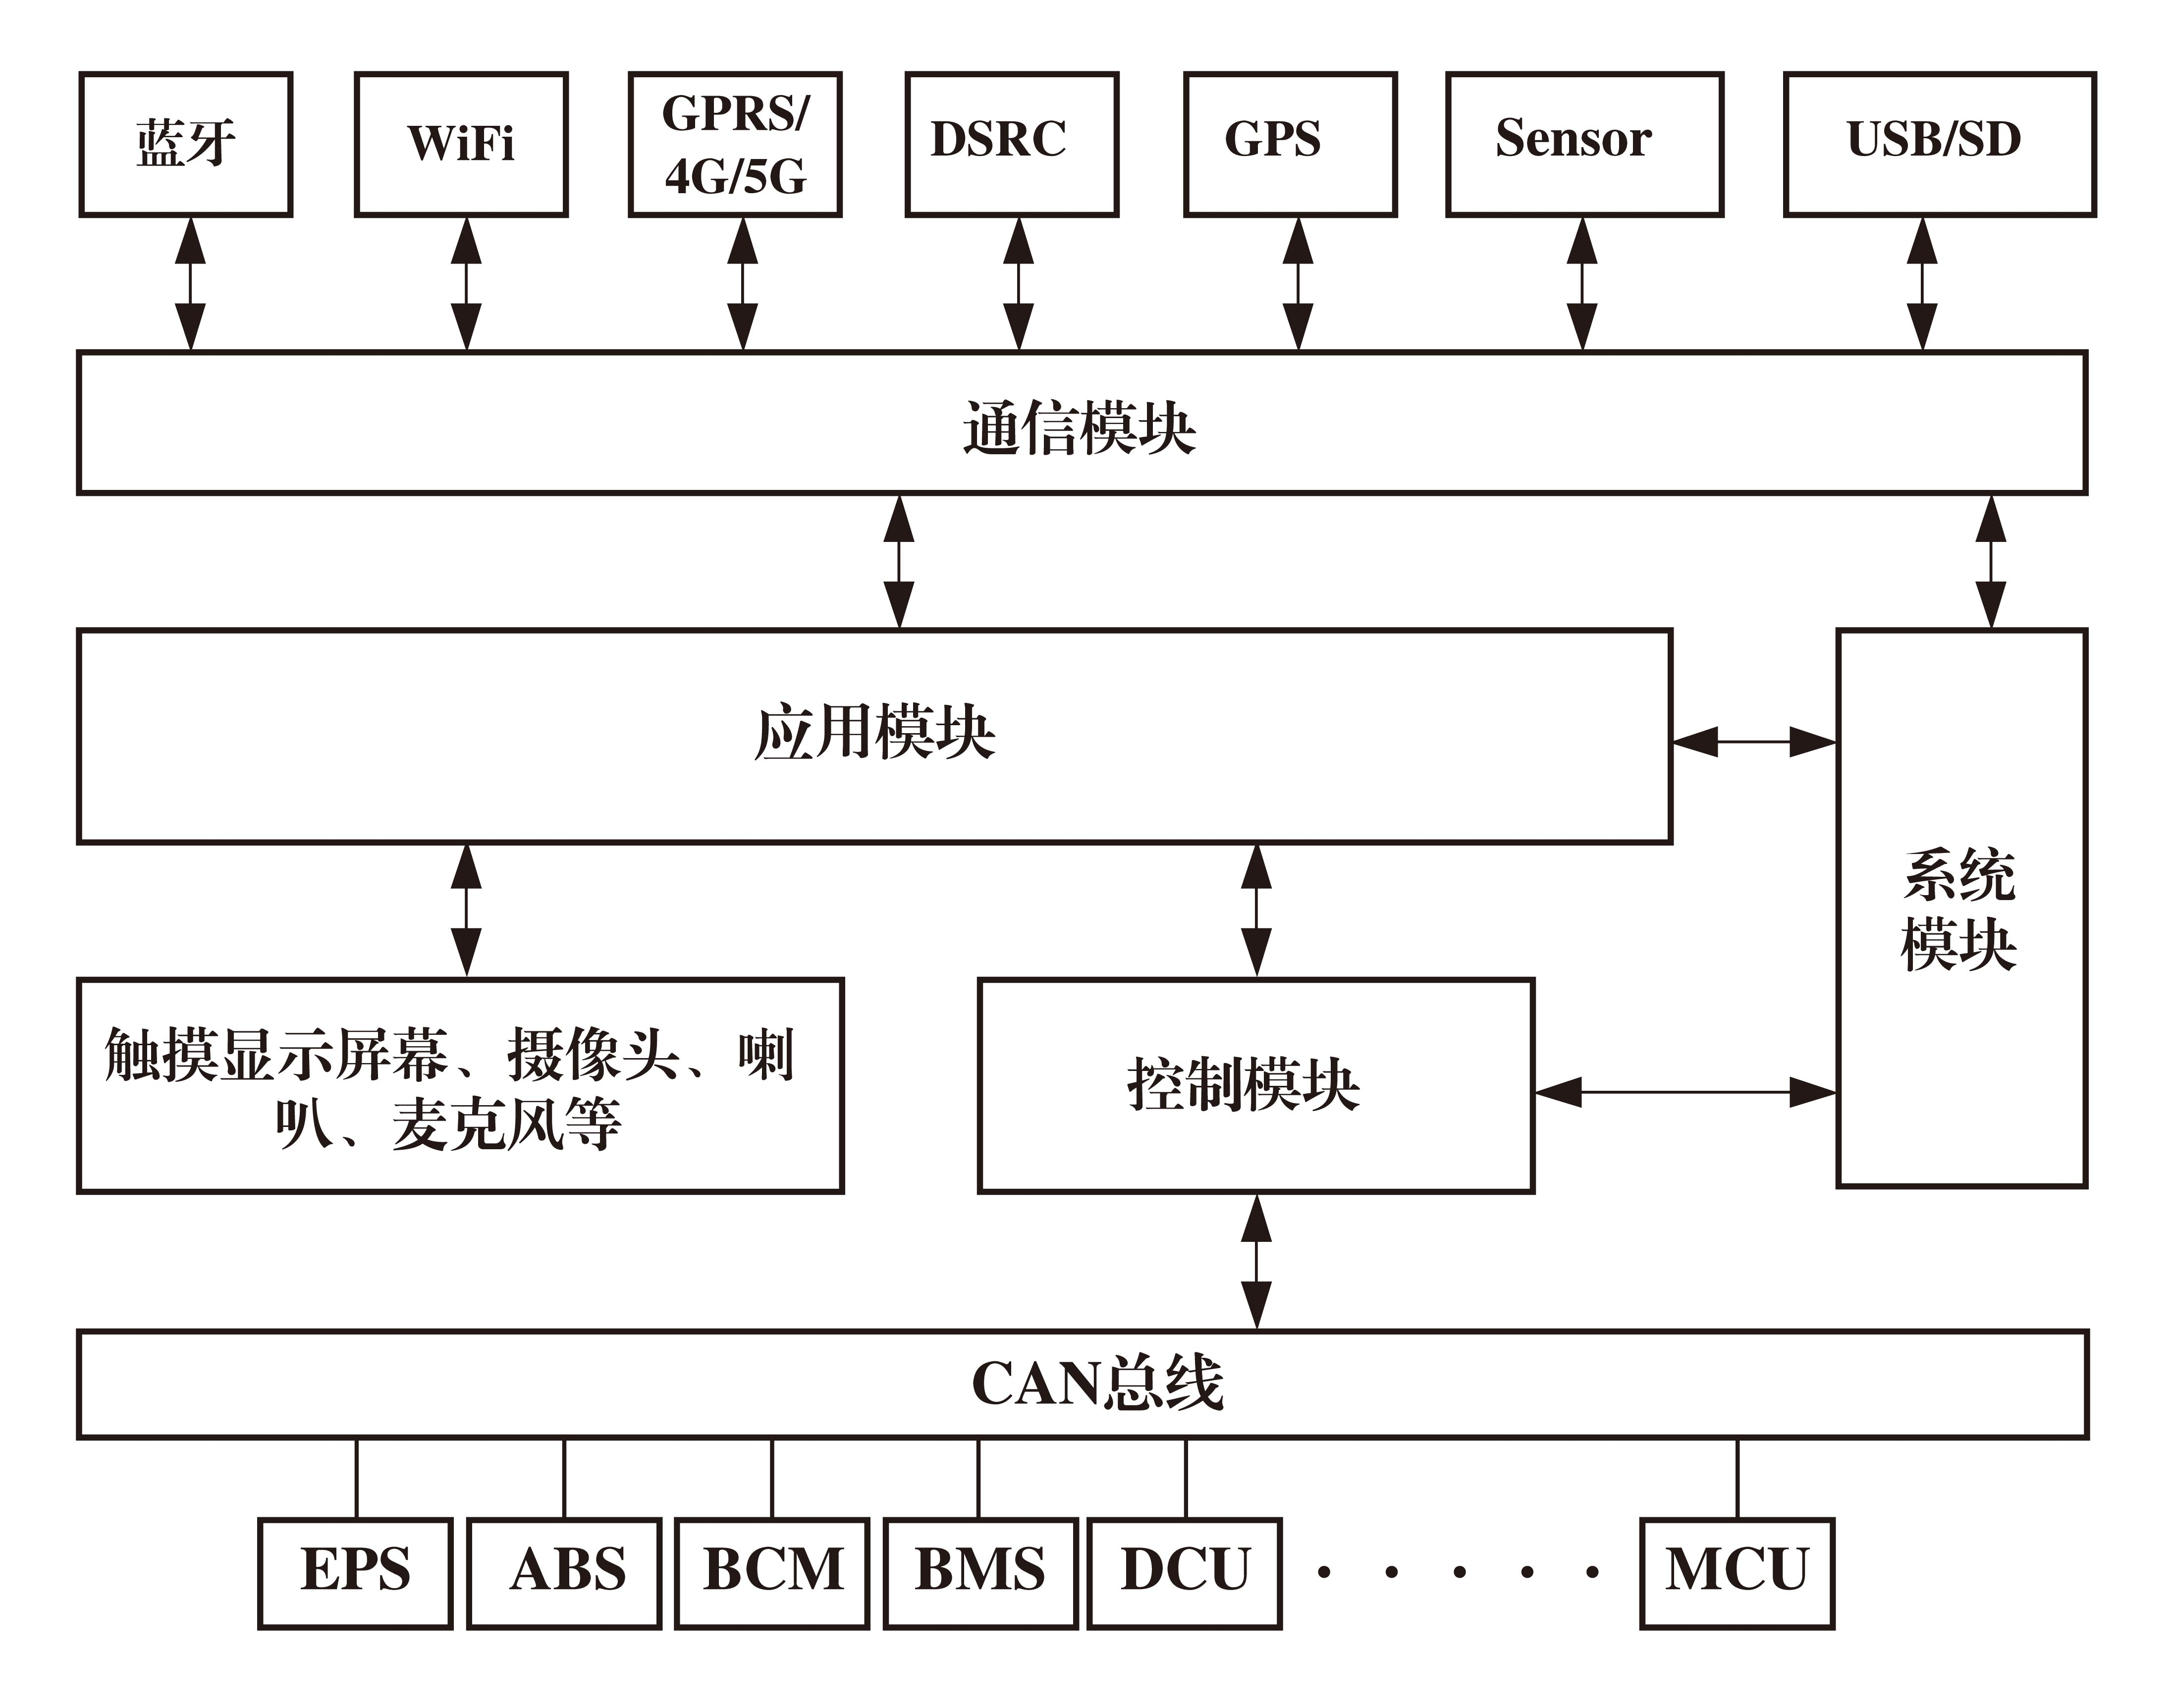
\includegraphics[scale=0.4]{resources/img/a50.jpg}
  \caption{IVI系统基础模块结构}
\end{figure}
该控制模块是车辆总线网中的一个节点点, IVI系统采用了基于车辆总线网的控制模块,完成了车辆的控制命令和车辆的数据采集。IVI系统在收到来自诸如手机 APP、 TSP服务等的控制端的控制命令后,向该控制单元传送该控制命令,该控制单元在收到该控制命令后,将该控制信息通过该车载总线传输该控制信息,从而完成对该车辆的控制工作,该控制模块能够将该控制运行的信息反馈给该控制端装置。传统的控制方法有:汽车启动控制、车门解锁、天窗控制、空调控制、车灯控制等;汽车信息包括:车窗状态,车门状态,车灯状态,胎压状态,燃料状态,位置信息,车速信息,汽车诊断信息等;和异常车门开启,胎压下降,汽车碰撞等。
本系统的功能包括电源管理、运行监控、故障诊断、下线检测等功能,以及通信、控制、应用等功能。IVI系统中的一个关键部件是:在 IVI中,它可以在 IVI中部署、在 IVI中的各个功能软件,如:信息娱乐软件、车身控制软件、汽车信息显示软件、行车安全监控软件等。

\section{IVI系统的安全风险分析}
通过对 IVI系统外部网络环境、内部网络结构、应用运行平台、业务功能服务等方面的分析,认为 IVI网络的安全性因素主要有:外部通信实体、无线通信网络、车载物理设备、 IVI操作系统、 IVI应用服务、 IVI应用数据、车载总线网络等。

(1)外部通信实体安全风险

在车辆网络中,外部通讯主体主要有移动终端设备、 TSP服务平台和智能网联车辆等。汽车网络应用中的移动终端设备、 TSP云服务平台、其它智能网联汽车等都可能受到病毒、木马或病毒攻击的威胁,从而影响到移动终端设备、云服务平台等与 IVI平台之间的安全信息交换。一旦恶意代码植入了一个终端装置或者一个业务平台,那么 IVI与该病毒的连接就会被恶意程序所入侵,并被恶意程序植入或者攻击,从而引起 IVI的恶意代码攻击,进而引起 IVI系统的故障,进而触发 IVI入侵车辆的总线。另外,一旦入侵方对其进行了入侵,就可以对 IVI进行欺诈袭击。

(2) 无线通信网络安全风险 

IVI系统一般集成了多种形式的无线通讯业务,如蓝牙, WiFi,蜂窝网络,车钥匙信号, GPS等,但由于其自身的安全性,使得它很可能是车辆的攻击对象。
由于无线通讯网中的通讯通道是非常开放的,而不同的无线通讯协定也都有其自身的安全性问题,使得通信链路上的攻击很可能会被攻破,或者是劫持、篡改、重放攻击;若不使用保密通信协定,则会造成资料在传送时受到攻击或损坏;此外,攻击者还可以对通信加密机制进行破坏,并对信号进行伪造访问。另外,黑客还可以使用虚拟的网路通讯技术,冒充网路实体来拦截车辆的无线电通讯资料,或是透过主动或消极地解析网路讯号,盗取使用者的合法资料。

(3) 车载物理设备安全风险 

其中, IVI系统的安全隐患是由 IVI系统所支持的硬件设施的安全性构成的,其中最大的安全隐患是由实体攻击造成的,其中包含了大量的内部总线、无线接入模块、其他适配界面(例如 USB (万能串行总线))等,并对汽车线路进行窃听、逆向等手段,从而获得 IVI的内部情报,从而进行进一步的进攻。然而,物理手段的实现比较困难,同时也给攻击者带来了巨大的危险,所以在本文中就不谈这种攻击的危险性了。

(4) IVI 操作系统安全风险 

当前 IVI系统的基础系统大都采用嵌入式 Linux, QNX, Android, WinCE等,但由于其自身的安全性,使得其具有一定的危险性。
1 系统越狱风险    
由于 IVI的版权和安全问题, IVI在生产前是完全关闭的,所以 IVI系统只能在工厂里安装 IVI,也就是在 IVI中安装了 IVI系统,也就是在 IVI中安装了 IVI系统,这个“繁琐”的操作,可以保证 IVI系统上的程序是经过了开发人员的签字和修改;另外,汽车业协会还对可供使用的应用程序进行了安全性测试,以保证 IVI和车辆使用者的信息的安全性。然而,这个封闭式的体系让很多的拥有者都被局限在了制造商的控制之下,而且有些程序的运行还得另外付费。于是,有些车主为了脱离车商的制约,会利用某些开源的越狱工具对 IVI进行系统的越狱,从而获得 Root的系统许可,免费安装各类应用程序,然而自由和自由的行为也会造成 IVI系统的安全性隐患。

(a) 系统稳定性降低。系统的越狱会对系统的稳定产生一定的干扰,从而提高系统死机、应用程序闪退、程序故障等问题。

(b) 信息安全隐患。在越狱后,可以提高操作系统的运行能力,可以读写根库,并对系统的文档进行控制,从而为入侵行为创造有利的环境。比如,当用户在越狱之后,可以通过软件的安全机制,下载很多“来历不明”的未经安全检查的未经许可的第三方软件,还有很多功能强大的外挂,这些外挂会对系统的安全和隐私造成一定的威胁,比如可以下载到关键的程序,比如修改系统的文件,导致车辆无法正常工作,从而导致车辆的安全问题。 

(c) 系统固件升级问题。一旦系统发生故障,系统很有可能会因为 OTA 而发生故障。
2 系统漏洞风险    
由于操作系统的软体设计有问题或有问题,会导致系统的漏洞。目前,网络安全漏洞是入侵操作系统的重要手段,其危害的范围非常广泛,不仅涉及到系统本身,还会对支持其正常工作的各类应用程序产生一定的冲击。若有黑客恶意地利用该漏洞,会对该系统产生不良的后果,比如植入木马、病毒等,盗取关键资料、修改系统档案、修改使用者资料、干扰系统的正常运作,并以此为契机,侵入到其它电脑上的应用程式也将受到同样的威胁。此外,对于曝光的系统安全问题,厂商也将适时地公布相关的补丁进行修补。但是,这些漏洞很有可能会有新的漏洞被发现,而新的漏洞也会随着时间的推移而不断的被发现,从而导致 IVI系统的漏洞越来越多。

(3) OTA 升级风险 

IVI系统和它的应用软件在初始的设计和发展中并不是十全十美的,所以它会出现很多问题,比如功能(系统功能的增强)、安全方面(系统和应用中的缺陷和 BUG)、性能(系统的资源优化),这些都要求 IVI系统和它的软件供应商通过改进系统和应用来处理这些问题。
IVI系统的传统更新方法有两个,一是直接驾车到维修中心进行更新,这样虽然更安全,但不方便,也不及时;丰田,大众,福特,沃尔沃,通用,特斯拉等公司纷纷利用 OTA技术,对 ECU、 IVI系统、车载应用软件进行 OTA升级。
OTA升级过程中的安全问题包括云服务器安全、汽车端安全、车与云通信安全,其中包括升级过程中的劫持、升级包文件篡改、升级包签名私钥泄露、升级包加密加密等安全问题。

(4) 非授权安装风险 

IVI系统仅能使用厂商或 IVI系统的厂商所许可的软件或更新软件,以确保 IVI的安全与保密。一来,使用者可以越狱获得系统的权限,来安装各种未经许可的程序。另外,安卓的一些应用则采用了 Debug版本的标识,这个标识由安卓 SDK公布,可以从某些途径获得,并模仿出一个系统的应用。通过签署的方式,可以通过使用未被许可的软件来进行安装,因为它们会对使用者的隐私和车辆的安全性造成威胁。 

(5) IVI 应用服务安全风险 
IVI软件的安全性是指在 IVI基础上,在 IVI基础上的所有应用软件的安全。随着汽车网络的服务能力的发展,汽车上的各种应用软件都具备了网络的能力。这类软件是针对智能联网车辆进行远程打击的主要手段。

(1) 应用程序漏洞风险 
就像是一个系统漏洞,软件漏洞也很大程度上是因为软件的逻辑结构的缺陷,错误的原因,比如应用程序的操作中的错误,比如,软件的运行中的不安全的部件,比如编程时的安全漏洞,编码的隐患等等。安全问题包括代码安全,数据安全,业务逻辑安全,系统环境安全,集成插件安全等。
利用弱点是入侵软件最常用的方法。恶意或不自觉地利用应用漏洞,会对应用系统造成很大的威胁,比如黑客通过软件的弱点入侵到应用系统中,获取应用系统的控制权,然后在应用系统中植入木马、病毒等手段,对应用软件进行入侵、入侵、入侵、盗取关键文件、修改用户的数据、干扰系统的正常使用等。而攻击者则会以此为突破口,通过 OS的弱点入侵 IVI系统。即使是内置的汽车联网,也能造成更大的危害。根据现有的缺陷,软件中的缺陷要比在操作系统中的要大得多。

(2)软件篡改风险 
通过反编译、反分析、篡改源代码、注入各种恶意代码来进行入侵。因为许多应用程式的开发人员没有足够的精力去防止反编译和篡改,也没有足够的技术,比如安卓的开放,还有许多常见的反编译和篡改技术,都是非常的容易的。通过反编译、反向分析,可以很容易地分析出所采用的通讯协定及资料的密码方法。
签名和检查是保护程序安全的重要手段,但是,由于该系统中的一些缺陷会使攻击人员绕开该密码,从而使攻击人员能够篡改程序。当黑客在服务供应商的应用程序商店或者第三方程序市场上发布了带有恶意代码的盗版程序时,可以取代原来的程序进行公开下载和更新。一旦使用者使用被恶意修改的程序,将会面临帐号、密码、文件、照片等隐私信息的泄漏,并且一旦被感染,将会被遥控。 

(3) 第三方 SDK 安全风险
第三方 SDK (Software Development Kit)典型地是第三方的软件供应商,例如广告商,社会平台,支付公司,推送平台等,为了便于应用开发者的使用,开发了一套软件工具箱, SDK用于包装对应的业务逻辑实施和服务要求和应答(API)。SDK是一种具有脆弱性的软件,其安全性问题会对其所用的应用系统的安全性产生直接的威胁。SDK应用广泛,其影响的领域广泛,其安全性的危险是显而易见的。 

(a)一个具有攻击性的 SDK自身构成了一个安全性的危险,这些软件可以窃取用户的私密资料而不被用户察觉,即使是在软件中,也有一些对 SDK的控制;另外,还有一些不怀好意的 SDK会在运行时进行动态的下载,并会在某些程序中安装恶意程式。

(b) SDK本身有一个软体安全性缺陷,可以让攻击者利用它来对 SKD本身的功能和所用的应用进行恶意的攻击。

(c)一些 SDK利用非保密通讯协定来传送资讯,比如透过 HTTP (超文字传送协定)明文传送秘密资讯,或是接受来自伺服器的命令与程式,以及执行程式的动力负载程式,为攻击者提供偷盗与居间攻击的可能。

(4) 非授权访问风险 

IVI应用程式若有安全性问题或权限验证等问题,可能会造成 IVI程式不受许可的使用而造成威胁,而另一端则可能造成使用者不受许可而进入其程式。而黑客则可以伪装成正当的使用者,绕过应用程式的存取控制,非法地操纵和利用程式的网路资源和资讯,或扩充其权限,或超越其权限,取得更多的资料。

(6) IVI 应用数据安全风险 

IVI系统一般包括车身控制,辅助驾驶,故障检测,导航定位,交通信息,移动办公,无线通讯,在线娱乐和 TSP等应用程序,其中包括汽车运行数据、汽车车主信息、汽车定位信息、车载应用系统数据等。IVI系统漏洞,应用程序漏洞,病毒和黑客入侵都会导致 IVI系统应用程序的资料遭到篡改、破坏、删除等行为,一些不经许可的应用程序和使用者可以存取一些机密资料,从而导致机密资料泄露。IVI系统的数据处理存在如下的安全性问题。
(a)外部安全威胁。而在 IVI系统中,黑客则通过 IVI系统漏洞、 IVI软件漏洞以及自身的安全漏洞来对 IVI系统数据、业务数据或数据库进行攻击。在系统的外部安全性方面,有未授权的应用,未授权的用户,未授权的数据访问,数据库通信协议的漏洞,系统平台的漏洞,认证的漏洞。 
(b) 内部安全威胁。如果使用者不小心存取机密资料,或不小心更改或移除资讯或使用者为未经许可之备份,则可能造成安全性危险。
(c) 共享数据。IVI操作系统、核心应用程序、通用应用程序共享的数据存贮器、共享共享、共享共享等多种形式的文件,导致了对系统和核心重要信息的恶意入侵;系统数据和隐私数据的明文保存也存在着数据泄漏的安全性问题。
(d) 合作伙伴。针对车辆使用程序的弱点,以应用程序作为平台,对车辆的敏感资料和个人信息进行了有效的防护,比如:过度使用、非法使用、授权升级、认证不充分等。 

(7) 车载总线网络安全风险 

一些厂商所开发的车辆联网系统,有些以 IVI为总线结点,与车内的资讯娱乐总线上直接相连,有些则是将 IVI系统与车用网关直接相连,这样做既会把 IVI系统的安全隐患带入到车上,又会对车辆的安全造成一定的威胁。
 
从上述的网络安全事故中可以发现,一些攻击是利用T-BOX和 OBDII的安全缺陷,对汽车的入侵进行了入侵,并对 IVI系统进行了入侵,从而获得了用户的隐私,从而使 IVI系统的内部通讯网络也可以作为攻击者的攻击途径,其攻击路线如下图2.2所示。
(1)在 IVI系统遭到入侵并被入侵后,攻击者可以通过 IVI监听汽车内的车辆信息,通过读取 CAN总线及专用通信协定,获取车辆状态信息、车辆状态信息、控制指令等信息。并可利用 IVI作为一个平台,实现对车辆进行更有威胁性的攻击,实现对车辆的遥控。
(2)针对汽车总线网的网络安全问题。由于现有的 CAN总线协议安全漏洞、协议滥用、数据泄露和弱认证等安全漏洞,使得黑客可以监听总线传输的数据,并进行欺骗、重放和洪水袭击等。随着汽车网络系统中的 WOBD系统、T-BOX系统、智能传感系统等多方面的不断发展,汽车总线系统所面临的安全问题日益突出,一旦有一个系统遭到了入侵,那么它就会成为 IVI系统的一个踏脚石。例如T-BOX的安全性问题,其主要包括汽车 OBD设备、手机 APP以及 TSP服务等, OBD设备既要与手机或 TSP业务进行数据交换,因此 OBD设备自身也会受到类似 IVI的威胁;另外, OBD装置还必须与其它车辆进行 CAN总线通讯,以达到多种车辆及遥控业务的目的,所以若有黑客入侵,则会对 IVI系统的安全性造成一定的损害。

\section{基于STRIDE的IVI威胁建模实例}
由于在第四章提出的威胁建模风险评估模型是基于传统的STRIDE模型来的, 因此本节将通过传统的STRIDE模型对智能网联汽车车载娱乐系统IVI进行威胁建模,并以此为例对此进行风险评估
为后续的新型风险评估模型进行前置理论基础。

我们从内部环境和外部环境视角,对 IVI系统的攻击面和安全威胁进行了全面分析。
在此基础上,建立了 IVI系统的安全威胁建模模型如图3.2。
在 IVI 安全威胁方框模型中,以虚线为代表,上层为框图。
其中,最小的是外部实体,最小的是在方框图模型的底部。
在进行通讯时,通过的信任边界数目越多,其所面临的安全性风险也就越大。

\subsection{车载IIVI系统的STRIDE威胁模型}
威胁识别是对信息系统划分的各个数据流构建STRIDE
威胁建模,分析每个数据流及其关联的资产是否容易受到S、 T、R、I、D以及E类威胁的攻击,识别并记录这些威胁。该IVI系统数据流的STRIDE威胁模型如图3.2所示。
\begin{figure}
  \centering
  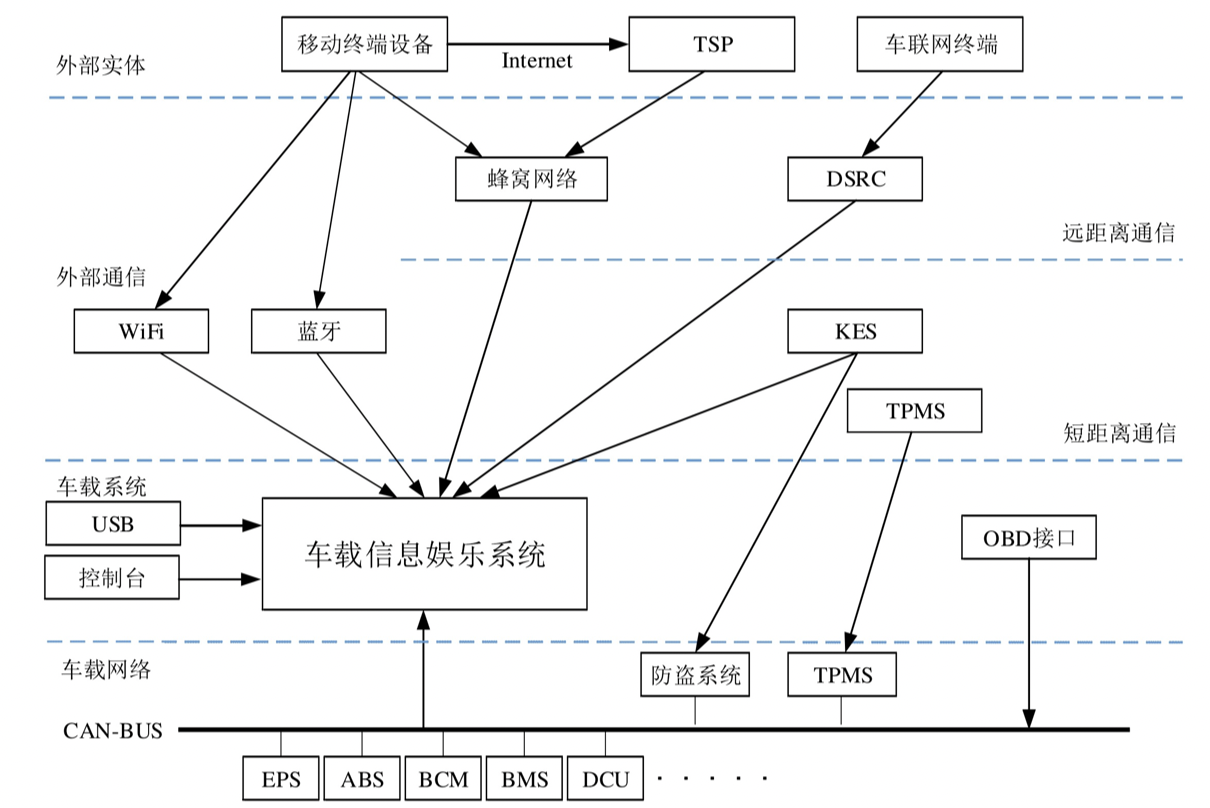
\includegraphics[scale=0.6]{resources/img/i33.png}
  \caption{车载娱乐IVI系统安全威胁建模图}
\end{figure}
\subsection{DF数据流威胁描述}
这里我们对三个外部元素:WIFI, USB, GPS 进行威胁评级描述分析
并把它们的数据流分别称为: DF1, DF2, DF3。

(1)DF1 WIFI与智能网联汽车IVI车载娱乐系统交互
该数据流可能面临的威胁有:攻击者通过劫持路由器伪装Wi-Fi信号, 窃听用户传输信息\cite{berghel2005wifi}

(2)DF2 USB与智能网联汽车IVI车载娱乐系统交互
该数据流可能面临的威胁有:通过USB设备的固件进行重新编程,来执行恶意行为,比如恶意文件下载、数据泄露等\cite{nissim2017usb}。

(3)DF2 GPS与智能网联汽车IVI车载娱乐系统交互
该数据流可能面临的威胁有:通过对搭载GPS传感器的车载信号接收器发送虚假信号, 从而误导汽车导航定位等\cite{alamleh2020cheat}。
\subsection{威胁评级}
我们通过STRIDE的五个属性即第二章提到的威胁评级给这实体威胁进行评分:
Wi-Fi 信号,潜在损失 D,可获得很多信息,所以评分为 3;重现性 R,Wi-Fi 可重现
性较强,评分为 3;可利用性,路由器的设置也极为简单,评分为 4;受影响用户 A 影响的一般是普通用户,评分为 2;
可发现性,较为容易发现,评分为 2。再根据评级公式,可得出威胁评级 Rank = (3 + 2 + 4 + 2 + 2) ÷ 2 = 6.5。
USB,潜在损失 D,可获得很多信息,所以评分为 3;重现性 R, 可重现
性较强,评分为 3;可利用性,由于要进入车体连接USB较难实现,可利用性低评分为 1;受影响用户 A 影响的一般是普通用户,评分为 2;
可发现性,较为容易发现,评分为 2。再根据评级公式,可得出威胁评级 Rank = (3 + 2 + 4 + 1 + 2) ÷ 2 = 6。
GPS,潜在损失 D,可获得很多信息,所以评分为 3;重现性 R, 可重现
性较低,评分为 1;可利用性,由于要通过伪造信号基站成本较高,可利用性低评分为 1;受影响用户 A 影响的一般是普通用户,评分为 2;
可发现性,较难发现,评分为 3。再根据评级公式,可得出威胁评级 Rank = (3 + 1 + 1 + 2 + 3) ÷ 2 = 5。
如表3.2我们给出了GPS的威胁列表
\begin{table}
  \caption{GPS威胁列表}
\begin{center}
    \begin{tabular}{|l|l}
      \hline 威胁编号 & A2 \\
      \hline 元素实例 & GPS \\
      \hline 威胁类别 & Spoofing \\
      \hline 威胁描述 & 伪装假GPS信号 影响用户GPS功能 \\
      \hline 威胁评级 & 5 \\
      \hline 消减威胁 & 升级GPS固件加固GPS信号和其他辅助导航软件 \\
      \hline
      \end{tabular}
  \end{center}
\end{table}

\section{本章小结}
通过研究智能网联汽车IVI系统中的安全问题,本文分析了 IVI系统在车联网环境下可能遇到的各种安全隐患。
结合IVI系统的实际应用情况及未来发展趋势,对 IVI系统的安全风险因素进行了全面分析。
对 IVI系统进行网络安全风险分析与评价,为 IVI系统的网络安全问题的深入研究和探讨。
最后本文通过对 IVI系统的功能结构的分析和总结,提出了基于 STRIDE的IVI威胁建模,最后给出了典型数据流的威胁评级。
